\section{Risk analysis}

La gestione dei rischi è quella disciplina che ha come obbiettivo l'identificazione, gestione e eliminazione dei rischi prima che quest'ultimi diventino una minaccia per il progetto. 

Che cos'è un rischio? Definiamo \textbf{rischio} come la possibilità che ci sia un danno. Bisogna cercare di prevenire un evento che può portare ad un danno serio. 

Definiamo \textbf{risk exposure}(RE), che è una grandezza (calcolabile), per calcolare quanto un progetto sia esposto ad un rischio. Viene calcolato come: 
$RE = P(UO) \cdot L(UO)$. Dove \begin{itemize}
    \item \textbf{P(UO)} è la probabilità di un \textit{unsatisfactory outcome}, ovvero la probabilità che effettivamente un danno (o comunque un risultato non soddisfacente) sia prodotto.
    \item \textbf{L(UO)} è l'entità del danno stesso, ovvero è la perdita per le parti interessate se il risultato non è soddisfacente.
    \end{itemize}
    
Definiamo \textbf{outcome unsatisfactory (\textit{risultato non soddisfacente})} come un risultato non positivo che riguarda diverse aree:
\begin{itemize}
    \item \textbf{utenti} come un progetto che presenta le funzionalità sbagliate, una UI carente, problemi di prestazioni o di affidabilità etc$\ldots$. In questo caso se i problemi sono gravi si hanno alti rischi, come l'utenza che smette di usare il prodotto, portando al fallimento del prodotto, o anche a conseguenze legali.
    \item \textbf{Per gli sviluppatori} con rischi che per esempio si ritrovano superamento del budget e prolungamenti delle scadenze impostate
    \item \textbf{Manutentori}, si possono ritrovare con dei componenti di qualità bassa software e/o hardware
\end{itemize}

Se abbiamo un rischio che produce un \textit{outcome unsatisfactory} il primo elemento su cui soffermarsi è lo studio degli eventi che abilitano il rischio, detti \textbf{risk triggers}. Questo perché per prevenire un rischio, quello che possiamo fare è andare a lavorare sui suoi trigger, fare così in modo che questo rischio non sia mai abilitato. I trigger non sempre sono facili da trovare. 

Quando parliamo dei rischi da un punto di vista della classificazione è utile distinguerne due classi principali di rischio.
\begin{enumerate}
    \item Quelli relativi al processo: Abbiamo dei problemi nel processo di sviluppo software (costi, risorse, tempi)
    \item Quelli relativi al prodotto: Ha a che vedere con il prodotto software, in questo caso possiamo pensare ai fallimenti riguardanti la qualità del prodotto (sicurezza, prestazioni etc$\ldots$) o la distribuzione dello stesso
\end{enumerate} 
    \textbf{Entrambe le classi possono portare al fallimento del progetto e quindi
  vanno gestite entrambe.}
  
Cosa possiamo fare per gestire i rischi? Ci sono due fasi per la gestione dei rischi:
\begin{enumerate}
    \item Risk assessment:  si lavora per identificare quelli che sono i rischi più importanti/rilevanti che devono essere controllati. In questa fase si hanno:
    \begin{itemize}
        \item \textbf{Risk identification} Identificazione dei principali rischi
        \item \textbf{Risk Analysis} analisi dei rischi identificati (tramite calcolo del \textit{risk exposure} e studio dei triggers).
        \item \textbf{Risk prioritization}, che consiste nella prioritizzazione dei rischi analizzati, per focalizzarsi sui più pericolosi per poi scalare ai meno pericolosi.
    \end{itemize} Alla fine, dalla fase di prioritizzazione, si produce una lista dei rischi. LA stessa lista entra nella parte di \textbf{Risk control}.
    \item Risk control e consiste, in primis, sul \textbf{risk management planning}, producendo piani di controllo di due tipi:
    \begin{enumerate}
        \item Di managment: gestione del rischio prima che il rischio si verifichi 
        \item Di contingency: cosa fare quando il rischio si verificherà. Questo succede qualora il \textit{piano di management} fallisca, ci serve quindi sapendo cosa fare a priori in caso di emergenza.
    \end{enumerate} si hanno anche due sotto-fasi per i due tipi di piani:\textbf{risk monitoring} e \textbf{risk resolution}.\\
    Le due fasi vengono ciclicamente ripetute perché i rischi, con il progredire dello sviluppo, variano.  
\end{enumerate}

\subsection{Risk identification}
Come facciamo a identificare i rischi che possono colpire un progetto? Una procedura complessa. 
Un modo per farlo potrebbe essere l'utilizzo di una \textbf{check-list}, includono un insieme di rischi molto comuni a molti progetti. L'analista scorre tale lista cercando rischi che possono essere applicati al progetto in analisi.

Alcuni rischi, in astratto, possono verificarsi sempre ma, il rischio che si sta considerando, va preso in considerazione solo per \textbf{ motivi specifici identificabili} nel mio progetto.\\
Alcune alternative alla \textbf{check-list}, possono essere le riunioni di confronto, \textit{brainstorming}, \textit{workshop} oppure il confronto con prodotti/organizzazioni correlate (confronto con prodotti simili). 

\subsection{Risk analysis}
Per analizzare i rischi si sfrutta esperienza delle reali probabilità che un rischio diventi realtà. Anche in questo si hanno degli schemi su cui basarsi: come \textit{modelli di stima dei costi}, \textit{modelli delle prestazioni}, etc$\ldots$ basati su \textit{simulazioni}, \textit{prototipi}, \textit{analogie con altri progetti} e \textit{check-list} (con stime di probabilità e danno).\\ Le stime sono molto specifici sul singolo progetto.

La parte dell'analisi dei rischi può anche implicare una analisi volta a prendere delle decisioni ai fini di minimizzare il risk exposure, scegliendo o meno tra varie opzioni, scegliendo in modo guidato dai rischi. Per farlo, possiamo utilizzare il decision tree, dove la radice dell'albero che rappresenta il problema. Successivamente andiamo a verificare i vari scenari e successivamente, per ogni scenario, andiamo a calcolare la probabilità che quel scenario si verifichi e poi andiamo a stimare il danno che quel scenario può causare. 

%\begin{figure}[H]
%  \centering
%  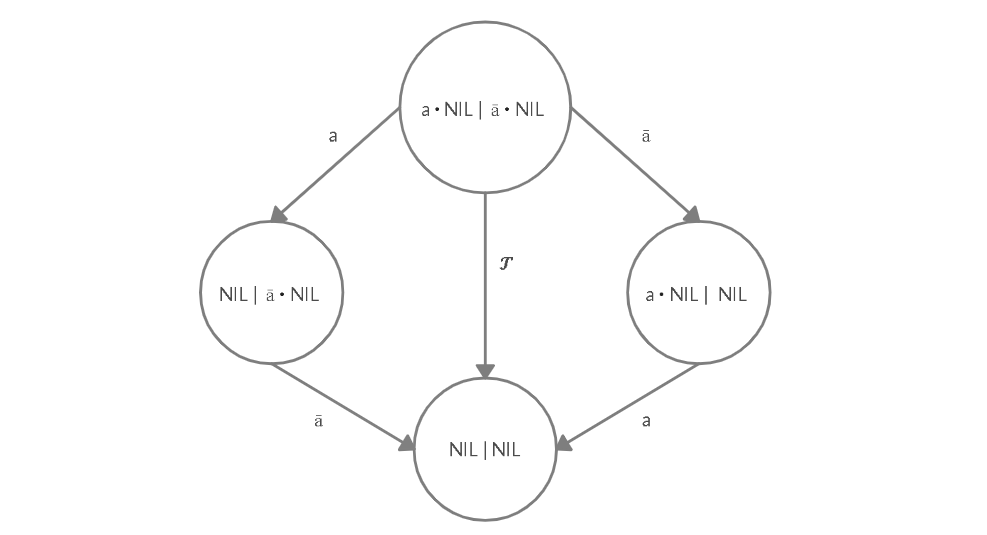
\includegraphics[scale = 0.2]{immagini/Cattura.PNG}
%  \caption{Esempio di decision tree}
%  \label{tree}
%\end{figure}

Si hanno di volta in volta i vari scenari, con le stime di probabilità di trovare un errore critico, di fallimento, di non trovare errori critici etc$\ldots$. Tali probabilità verranno usate per il calcolo del \textit{risk exposure} insieme ad un quantificatore di $L(UO)$ spesso pari all'effettivo costo che conseguirebbe al risultato ottenuto. Infine i vari \textit{risk exposure} di ogni caso vengono sommati per ottenere il \textit{risk exposure} finale.

Ragionando sulle cause dei rischi, andiamo ad analizzare il \textbf{Risk tree} (è uno strumento). Alla radice del \textbf{risk tree} abbiamo il rischio. Trovioamo successivamente una serie di nodi, ogni nodo rappresenta un evento/condizione che a sua volte può essere scomposto in eventi/condizioni fino ad arrivare ad eventi \textbf{foglia}. La scomposizione è guidata da due tipologie di nodi logici:
\begin{enumerate}
    \item \textbf{AND-node}: dove i figli di tali nodi sono eventi legati da una condizione logica \textit{and} (i nodi figlio devono tutti verificarsi affinché il nodo padre si verifichi come conseguenza): dove i figli di tali nodi sono eventi legati dal un \textit{or} (basta che si verifichi uno dei figli)
    \item \textbf{OR-node}
\end{enumerate}

Dato un \textit{risk tree} cerco le combinazioni di eventi atomici che possono portare al rischio, questo perché quello che noi vogliamo è lavorare su queste combinazione per fare si che non si verifichino. Per farlo si esegue una operazione di \textbf{cut-set tree derivation} ovvero, partendo dalla radice scendendo verso le foglie, si riporta in ogni nodo la combinazione (o le combinazioni) di eventi che possono produrre il fallimento. A questo punto si vanno a calcolare le varie combinazioni degli eventi foglia. Praticamente si deriva un insieme di eventi non scomponibili sulle combinazioni dell'\textit{and}.

\subsection{Risk Prioritization}
Bisogna innanzitutto capire da quali rischi partire. Per farlo si pongono(mappano) i valori di $P(UO)$ e $L(UO)$ in un range, per esempio, da 1 a 10, ricalcolando il \textit{risk exposure}. Una volta fatto si lavora in base al \textit{risk-exposure} (che può anche essere un intervallo se le probabilità o i costi sono in un certo intervallo). Una volta effettuato il mapping dei valori ed è stato calcolato il necessario, possiamo eseguire un plotting portando sull'asse y la probabilità di verificarsi di un rischio (\textbf{P(UO)}, sull'asse x l'entità del danno (\textbf{L(UO)}) e poi ogni stima (RE), se precisa diventa un puntino, altrimenti viene rappresentato come un segmento all'interno del plot.  \\
I dati rappresentati mi permettono di segnare delle curve, quest'ultime rappresentano l'entità dei rischi più pericolosi. 

\subsection{Risk Control}
Avendo capito come sono stati prioritizzazti bisogna capire come gestirli.
Per ogni rischio si va a sviluppare un piano di gestione di quest'ultimo, questo piano diventa un vero e proprio documento composto dalle seguenti sezioni:
\begin{itemize}
    \item cosa si sta gestendo 
    \item come mitigare il rischio e quando farlo
    \item di chi è la responsabilità
    \item come approcciarsi al rischio
    \item il costo dell'approccio al rischio
\end{itemize}
Ma cosa facciamo per gestirli? Anche in questo caso vengono utilizzate le check-list che contengono l'insieme di tecniche di risk-managment più comuni in base al rischio specifico. 

Ci sono però alcuni aspetti più generali da considerare:
    \begin{itemize}
      \item \textbf{Reduce risk likehood}: lavorare sulla probabilità che il rischio avvenga, sulla probabilità dei  triggers. Bisogna capire come diminuire la probabilità.
      \item \textbf{Avoid risk}: lavorare, nel limite del possibile, sull'eliminazione stessa del rischio.
      \item \textbf{Reduce consequence likehood}: lavorare sulla riduzione della probabilità di avere conseguenze al danno, non viene quindi ridotto il rischio, ma vengono ridotte le probabilità del danno.
      \item \textbf{Avoid risk consequence} lavorare, nel limite del possibile, sull'eliminazione stessa del danno conseguente al rischio.
      \item \textbf{Mitigate risk consequence} lavorare sul mitigare le conseguenze di un rischio, diminuendo l'entità
      del danno.
    \end{itemize}
    
Bisogna anche studiare le contromisure, da scegliere e attivare in base alla situazione. Si hanno due metodi quantitativi principali per ragionare quantitativamente sulle contromisure:
\begin{itemize}
    \item \textbf{Risk-Reduction Leverage}, si calcola quanto una certa contromisura può ridurre un certo rischio  secondo la seguente formula: $\displaystyle RRL(r, cm)=\frac{RE(r)-RE(\frac{r}{cm})}{Cost(cm)}$ \\
    Dove $r$ rappresenta il rischio, $cm$ la contromisura e $\frac{r}{cm}$ la contromisura $cm$ applicata al rischio $r$. Calcolo quindi la differenza tra \textit{risk exposure} del rischio $r$ e quella avendo considerando la contromisura $cm$. Divido il risultato per il costo della contromisura.\\ La miglior contromisura è quella con il RRL maggiore, avendo minor costo e maggior efficacia dal punto di vista del \textit{risk exposure}.
    \item \textbf{Defect Detection Prevention, DDP}
    Questo metodo confronta le varie contromisure, confrontando anche gli obiettivi del progetto, in modo quantitativo e fa un confronto indiretto producendo matrici in cui si ragiona in modo indipendente sulle singole contromisure e sui singoli rischi ma il risultato finale è un confronto tra tanti rischi e tante misure che possiamo prendere in considerazione contemporaneamente. Si ha un ciclo di 3 passaggi:
    \begin{enumerate}
        \item Elaborare la matrice di impatto dei rischi. Questa matrice calcola l'impatto dei rischi sugli obiettivi principali (presi in considerazione) del progetto. 
        I valori della matrice, ovvero $impact(r, obj)$ (che ha per colonne i rischi $r$ e righe gli obiettivi del progetto $obj$) variano da 0, nessun impatto, a 1, completa perdita di soddisfazione (e totale non raggiungimento dell'obiettivo indicato). Ogni rischio viene accompagnato dalla probabilità $P$ (likehood) che accada. Ogni obiettivo è accompagnato dal \textbf{peso} $W$ che ha nel progetto (la somma di tutti i pesi è pari a 1). 
        
        Si possono calcolare altri valori di sintesi. In primis la \textbf{criticità} di un rischio rispetto a tutti gli obiettivi indicati: \[criticality(r)=P(r)\cdot\sum_{obj}(impact(r, obj)\cdot W(obj))\] La criticità sale se sale l'impatto e se sale la probabilità del rischio.\\ Un altro dato è la \textbf{perdita di raggiungimento} di un obiettivo qualora tutti i rischi si verificassero: \[loss(obj)=W(obj)\cdot\sum_{r}(impact(r, obj)\cdot P(r))\]
        
        \item elaborare contromisure efficaci per la matrice elaborata. In questa fase si usa il fattore di criticità del rischio. Viene prodotta una nuova matrice con colonne pari ai rischi (con probabilità e criticità) e righe pari alle contromisure. I valori presenti nelle celle saranno le riduzioni di rischio di una contromisura $cm$ sul rischio $r$ ($reduction(cm,r)$). La riduzione va da 0, nessuna riduzione, a 1, rischio eliminato. \\
        Si possono calcolare altri valori di sintesi. Possiamo calcolare la \textbf{combineReduction}, che ci dice quanto un rischio viene ridotto se tutte le contromisure che abbiamo identificato sono attivate: \[combineReduction(r)=1-\prod_{cm}(1-reduction(cm, r))\] 
        
        Un altro valore è l'\textbf{overallEffect}, ovvero l'effetto di ogni contromisura sull'insieme dei rischi considerato: \[overalleffect(cm)=\sum_r(reduction(cm,r)\cdot criticality(r))\] si avrà effetto maggior riducendo rischi molto critici \item determinare il bilanciamento migliore tra riduzione dei rischi e costo delle contromisure. Bisogna considerare anche il costo di ogni contromisure e quindi si fa il rapporto tra effetto di ciascuna contromisura e il suo costo e scegliendo il migliore
    \end{enumerate}
\end{itemize}

Analizzando il \textbf{Managment and Contingecy Plan}, dove il managment plan che definisce le azioni per prevenire il rischio, e il contingecy plan che indica quello che dobbiamo fare qualora si verifichi il rischio. 

Si passa quindi al \textbf{risk monitoring/resolution}. Queste due parti sono tra loro integrate. I rischi vanno monitorati e occorrenza vanno risolti il prima possibile. Tutte queste attività sono costose e si lavora su un insieme limitato di rischi, una decina, in base alle risorse disponibili.
